\begin{frame}[t]{1D MOC Code}
    
    
    
\end{frame}

%%%%%%%%%%%%%%%%%%%%%%%%%%%%%%%%%%%%%%%%%%%%%%%%%%%%%%%%%%%%%%%%%%%%%%%%%%%%%%%%%

\begin{frame}[t]{Fixed Total Source}



\end{frame}

%%%%%%%%%%%%%%%%%%%%%%%%%%%%%%%%%%%%%%%%%%%%%%%%%%%%%%%%%%%%%%%%%%%%%%%%%%%%%%%%%

\begin{frame}[t]{Fixed Total Source}
    
    \begin{figure}[H]
      \centering
      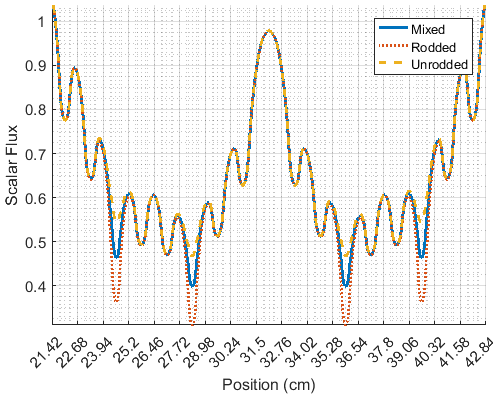
\includegraphics[width=0.7\textwidth]{../figs/1dmoc-50mix-fixedscat-scalflux7.png}
      \caption{Group 7 scalar flux comparisons for a fixed fission and scattering source calculation}\label{f:1dmoc-fixed-50-scalflux7}
    \end{figure}
    
\end{frame}

%%%%%%%%%%%%%%%%%%%%%%%%%%%%%%%%%%%%%%%%%%%%%%%%%%%%%%%%%%%%%%%%%%%%%%%%%%%%%%%%%

\begin{frame}[t]{Fixed Total Source}

\begin{figure}[H]
  \centering
  \subfigure[Group 1]{
    \centering
    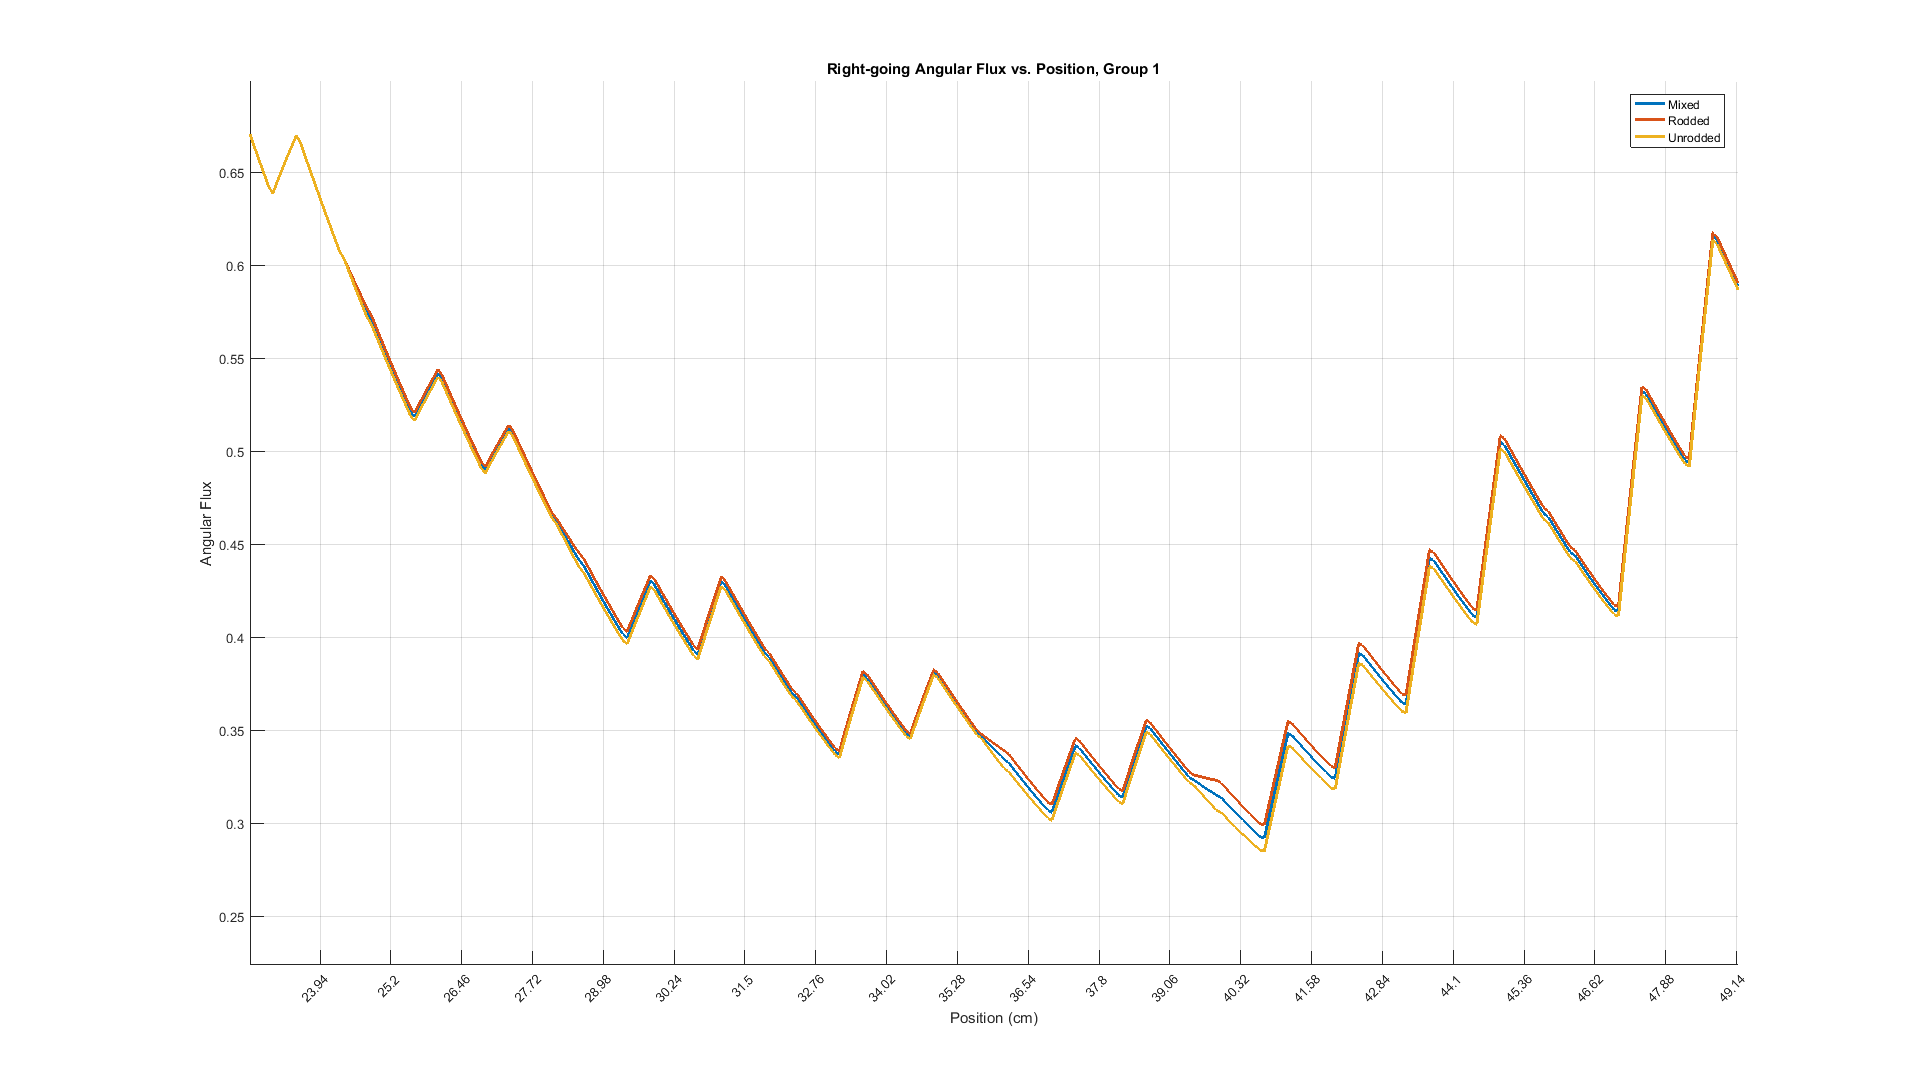
\includegraphics[width=0.6\textwidth]{../figs/1dmoc-50mix-fixedscat-angflux1.png}
    \label{f:1dmoc-fixed-50-angflux1}
  }
  ~
  \subfigure[Group 7]{
    \centering
    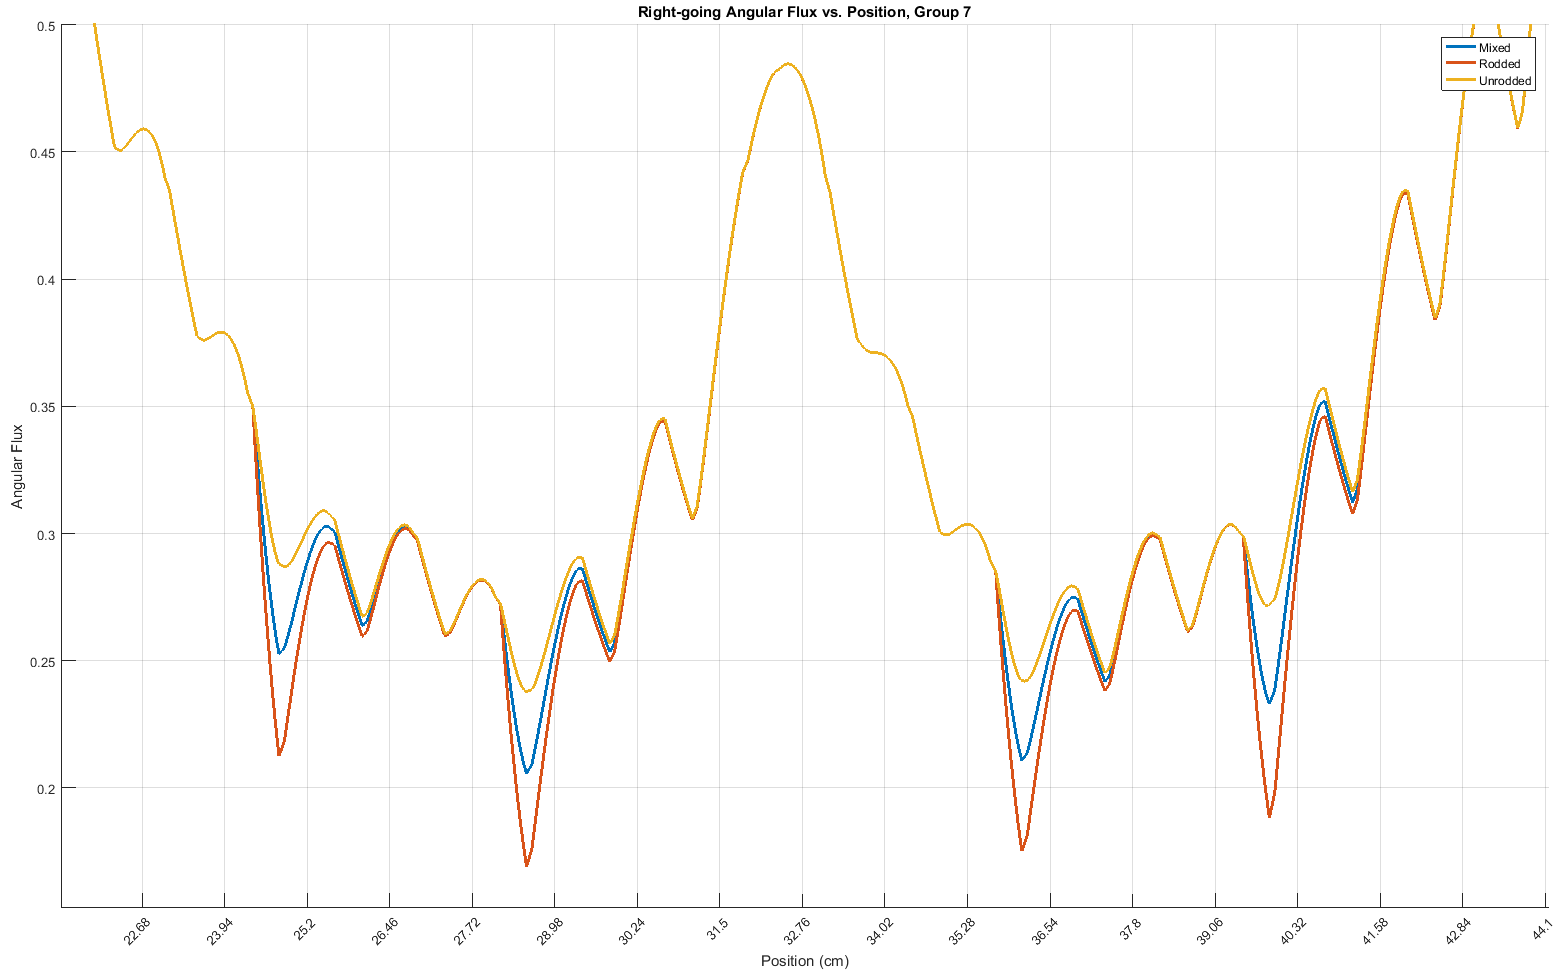
\includegraphics[width=0.6\textwidth]{../figs/1dmoc-50mix-fixedscat-angflux7.png}
    \label{f:1dmoc-fixed-50-angflux7}
  }
  \caption{Angular flux comparisons for a fixed fission and scattering source calculation}\label{f:1dmoc-fixed-50-angflux}
\end{figure}

\end{frame}

%%%%%%%%%%%%%%%%%%%%%%%%%%%%%%%%%%%%%%%%%%%%%%%%%%%%%%%%%%%%%%%%%%%%%%%%%%%%%%%%%

\begin{frame}[t]{Fixed Fission Source}
    
    
    
\end{frame}

%%%%%%%%%%%%%%%%%%%%%%%%%%%%%%%%%%%%%%%%%%%%%%%%%%%%%%%%%%%%%%%%%%%%%%%%%%%%%%%%%

\begin{frame}[t]{Fixed Fission Source}

\begin{figure}[H]
  \centering
  \subfigure[25\% Mixture]{
    \centering
    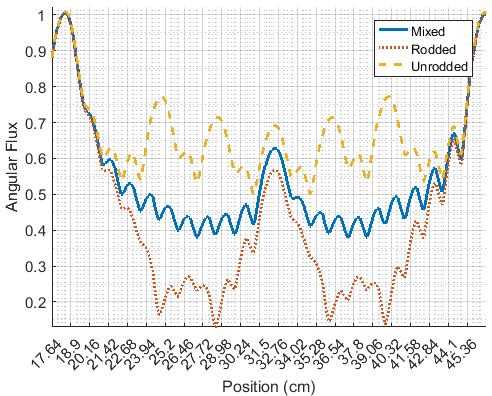
\includegraphics[width=0.45\textwidth]{../figs/1dmoc-25mix-angflux7.png}
    \label{f:1dmoc-25-angflux7}
  }
  \hfill
  \subfigure[50\% Mixture]{
    \centering
    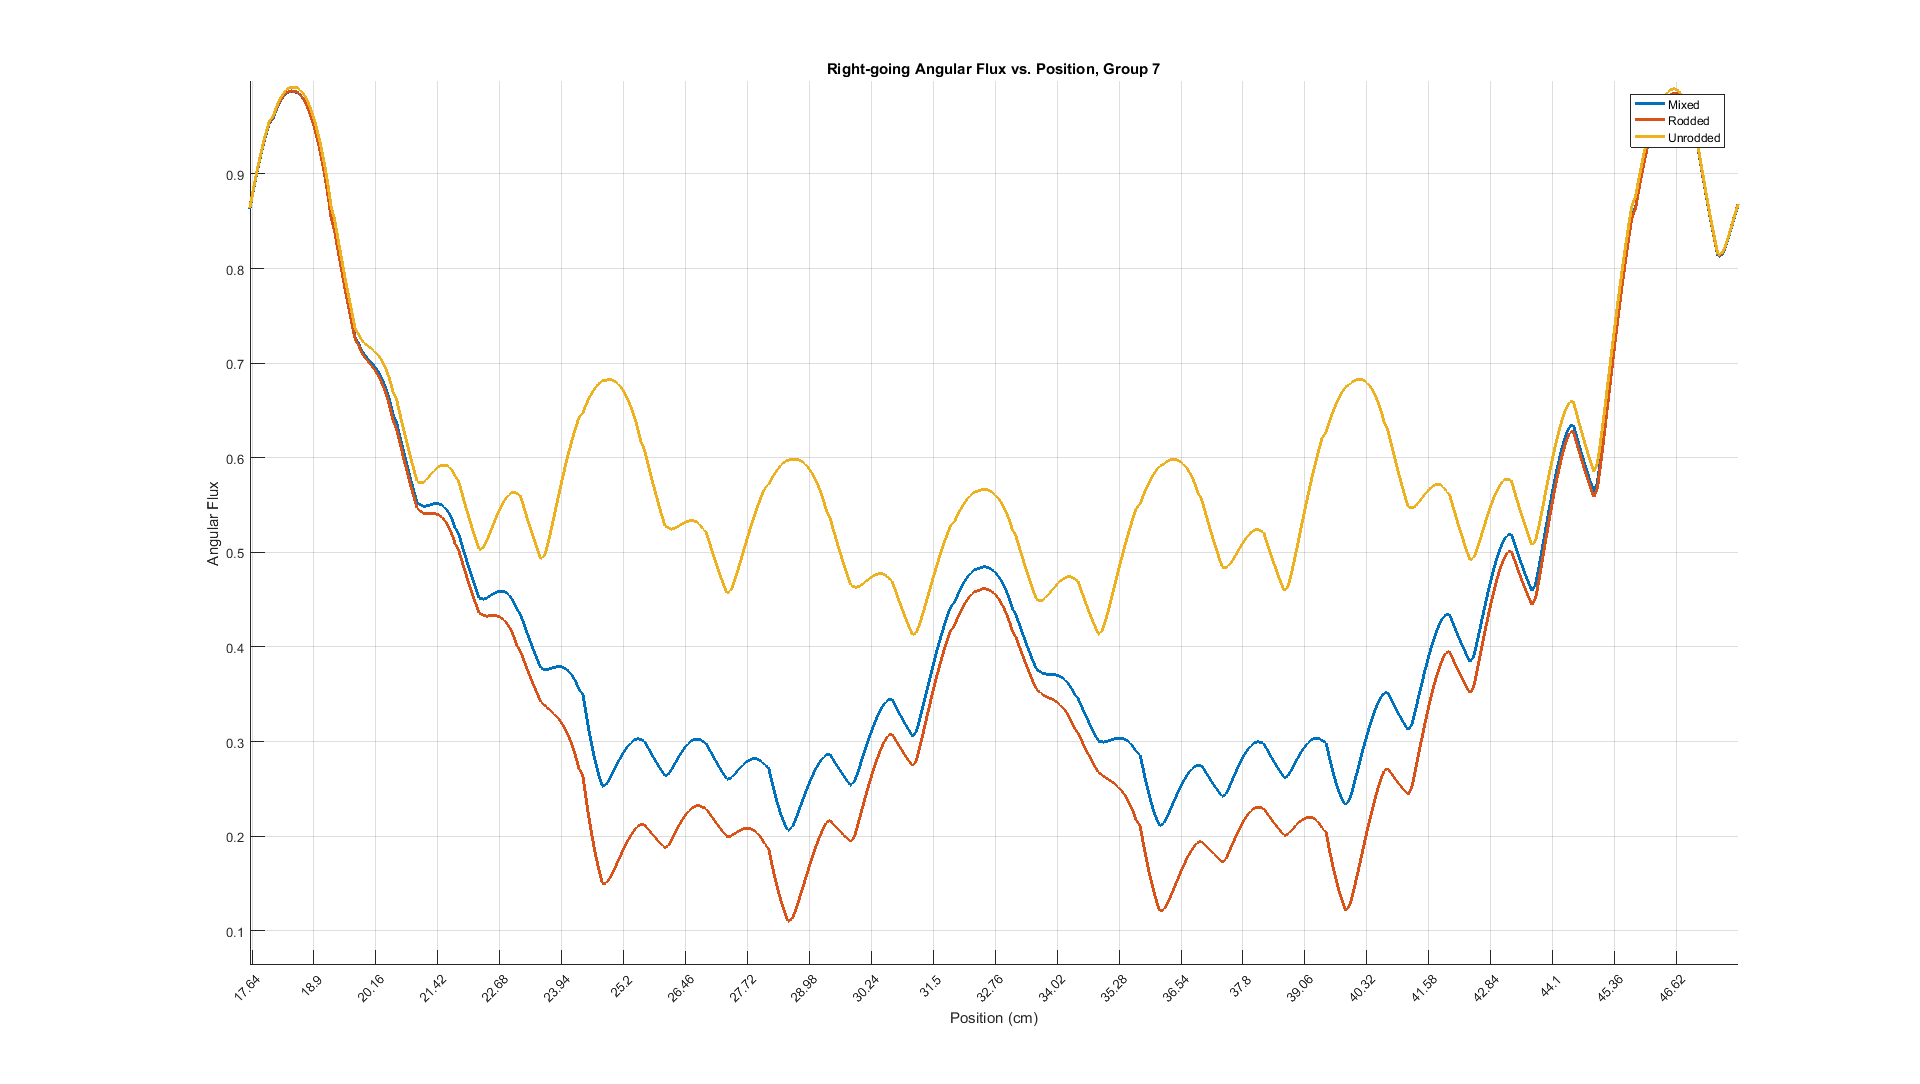
\includegraphics[width=0.45\textwidth]{../figs/1dmoc-50mix-angflux7.png}
    \label{f:1dmoc-50-angflux7}
  }
  ~
  \subfigure[75\% Mixture]{
    \centering
    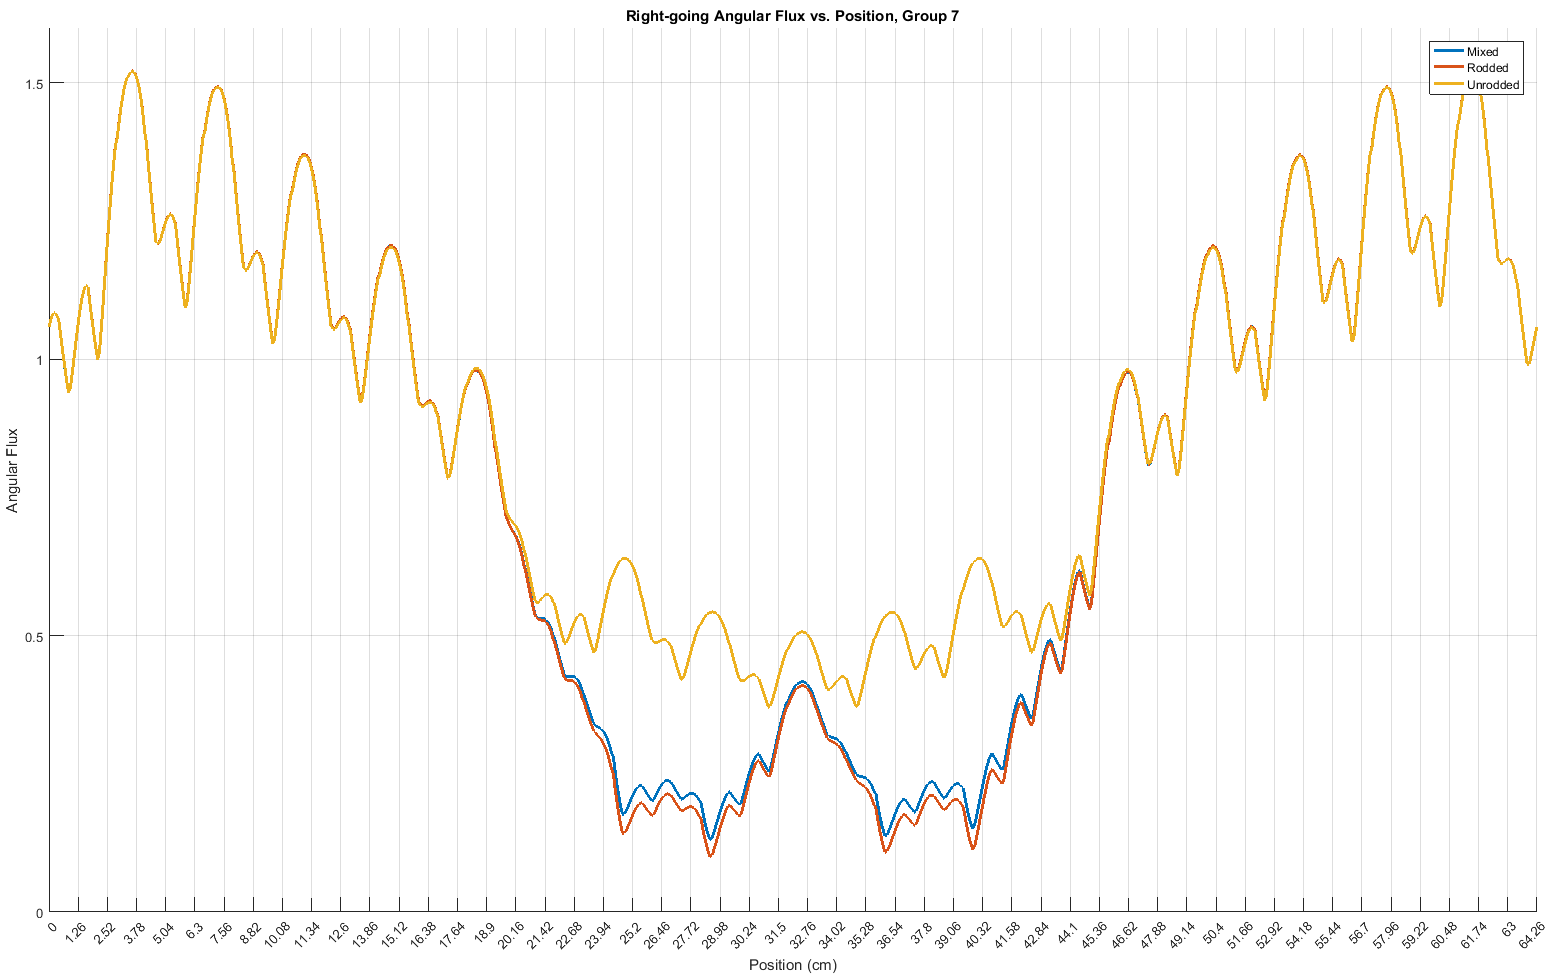
\includegraphics[width=0.45\textwidth]{../figs/1dmoc-75mix-angflux7.png}
    \label{f:1dmoc-75-angflux7}
  }
  \caption{Group 7 angular flux comparisons for 25\% and 75\% mixtures}\label{f:1dmoc-angflux7}
\end{figure}

\end{frame}

%%%%%%%%%%%%%%%%%%%%%%%%%%%%%%%%%%%%%%%%%%%%%%%%%%%%%%%%%%%%%%%%%%%%%%%%%%%%%%%%%

\begin{frame}[t]{Fixed Fission Source}

\begin{figure}[H]
  \centering
  \subfigure[25\% Mixture]{
    \centering
    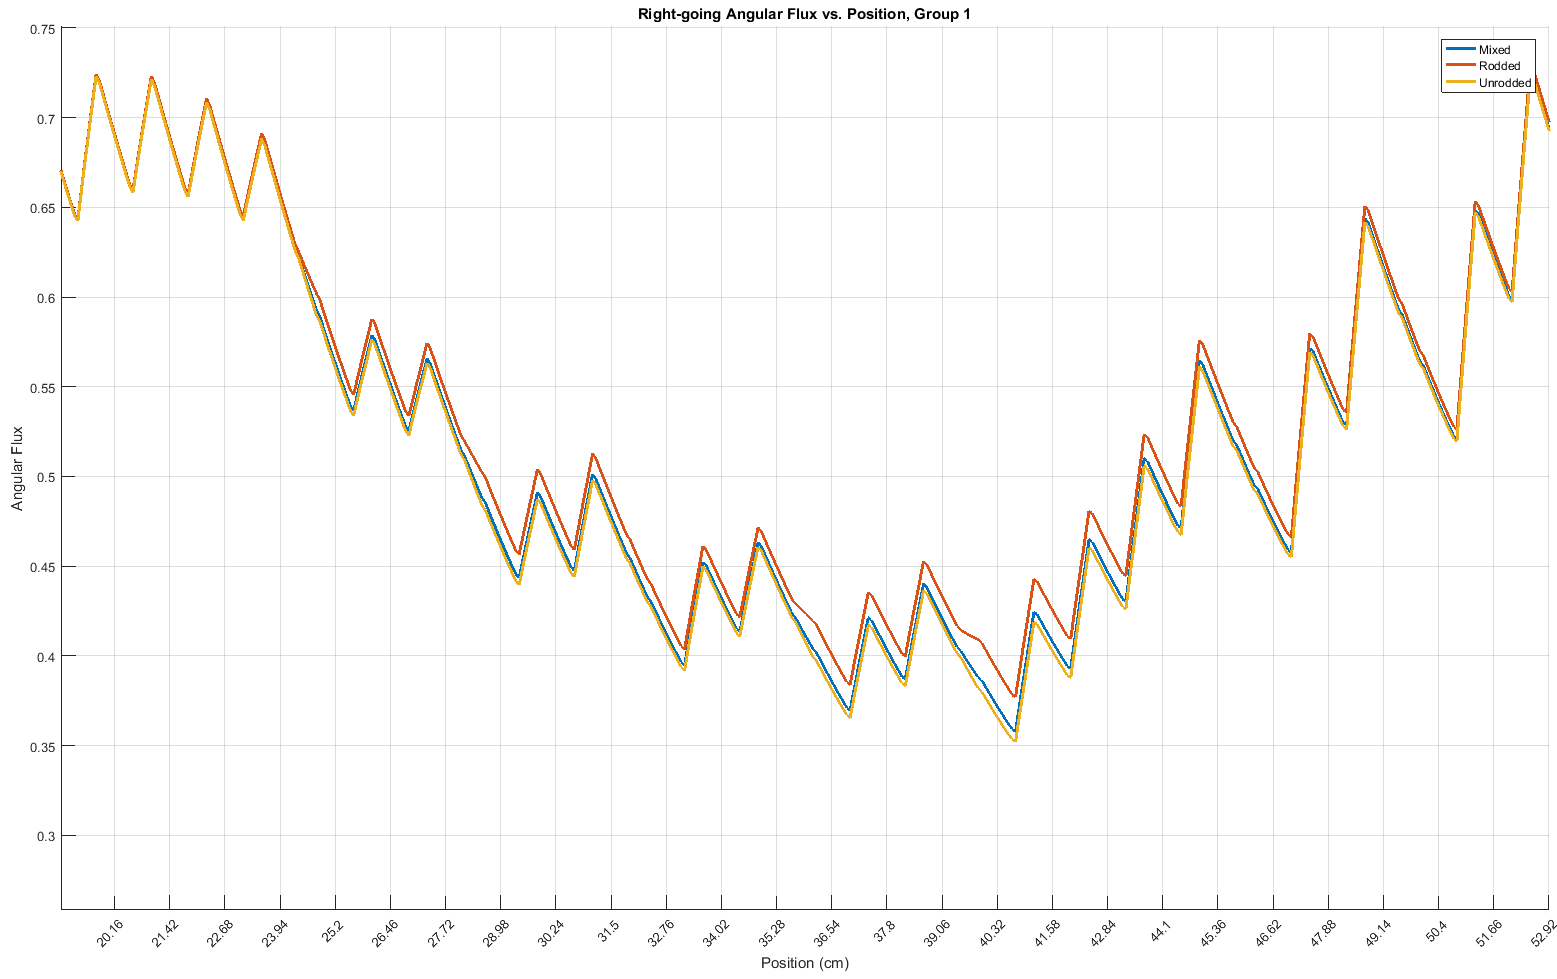
\includegraphics[width=0.45\textwidth]{../figs/1dmoc-25mix-angflux1.png}
    \label{f:1dmoc-25-angflux1}
  }
  \hfill
  \subfigure[50\% Mixture]{
    \centering
    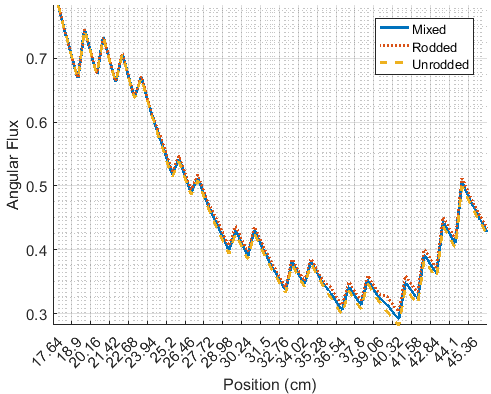
\includegraphics[width=0.45\textwidth]{../figs/1dmoc-50mix-angflux1.png}
    \label{f:1dmoc-50-angflux1}
  }
  ~
  \subfigure[75\% Mixture]{
    \centering
    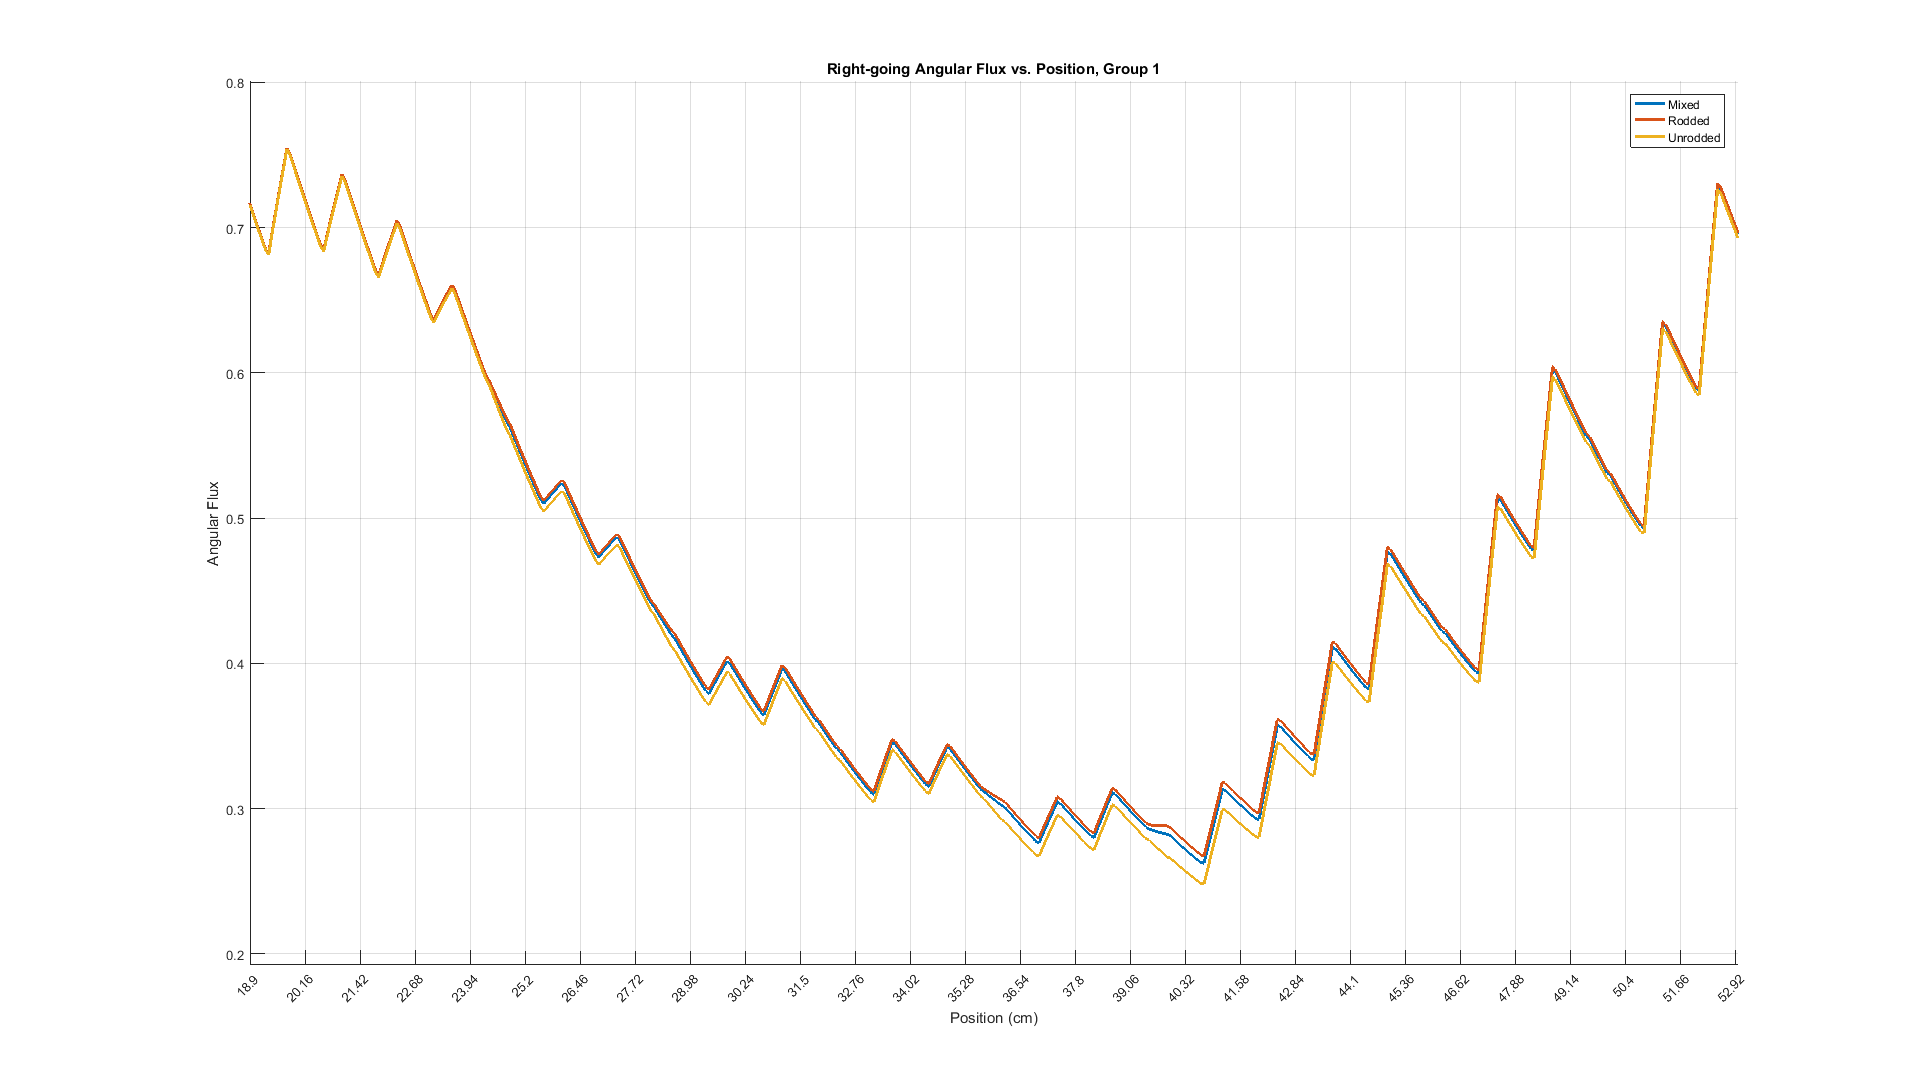
\includegraphics[width=0.45\textwidth]{../figs/1dmoc-75mix-angflux1.png}
    \label{f:1dmoc-75-angflux1}
  }
  \caption{Group 1 angular flux comparisons for 25\% and 75\% mixtures}\label{f:1dmoc-angflux1}
\end{figure}

\end{frame}

%%%%%%%%%%%%%%%%%%%%%%%%%%%%%%%%%%%%%%%%%%%%%%%%%%%%%%%%%%%%%%%%%%%%%%%%%%%%%%%%%

\begin{frame}[t]{Discussion}
    
    
    
\end{frame}

%%%%%%%%%%%%%%%%%%%%%%%%%%%%%%%%%%%%%%%%%%%%%%%%%%%%%%%%%%%%%%%%%%%%%%%%%%%%%%%%%

\begin{frame}[t]{Sub-Ray MOC Method}
    
    
    
\end{frame}